\chapter{Problem formulation}

Time series data connected to~diagnostic signals from the~industrial machines that are considered to~be faulty can be~divided into three main classes of~components:

\begin{itemize}
	\item component related to~the~ordinary operation of~the~machine or its expected operating conditions;
	\item damage-related component;
	\item background noise.
\end{itemize}

Operation-related component can be~understood differently with respect to~the~regarded machine. For stationary machines with rotating components, that are diagnosed by~analyzing their vibrations, it~stands for the~component being the~result of~the~machine kinematics. For other kinds of~diagnostic data (i.e. temperatures, pressures etc.), regardless of~the~type of~the~machine, deterministic component represents the~functional character of~machine's operation.

Fault-related component can be~understood in~a~more universal way. It can represent either information indicating change of~technical condition of~the~machine, or component present in~the~signal that is~not supposed to~be present, and can be~explained in~terms of~damaged component of~the~machine. 

Background noise can be~expected to~be present in~every real-life measured signal, however its character and meaning can be~different for every type of~investigated machine.

All of~described components are additionally influenced by~factors that can be~considered to~be external from the~point of~view of~individual machine components. Firstly, the~external load imposed on~the~machine is~a~randomly varying factor that introduces additional variance to~diagnostic signals that already have complicated structure. Another layer of~variability is~introduced by~the~influence of~environmental parameters. The most important are time-varying ambient temperature, also influenced by~the~air flow in~the~area. This factor mostly influences the~temperature data. On the~other hand, vibration measurements are heavily influenced by~disadvantageous noise characteristics. While researchers developing analytical methods very often assume stationary Gaussian noise, in~real-life industrial scenario it~is~typically not the~case. Especially for machines that experience process-related events of~random impacts (e.g. ore pieces falling into the~crushing machine), the~occurrence of~those is~a~non-Gaussian impulsive noise, that imposes difficulty for the~analysis of~such signal, especially when statistical methods are used. The existence of~those and other difficulties is~a~motivation for the~development of~dedicated analytical algorithms.

The described types of~information can be~carried outside the~machine in~the~form of~energy that is~wasted in~the~process that is~performed by~the~machine \cite{cempel2003holistyczne}. One can measure this energy in~various ways, typically in~the~form of~diagnostic signals measured using wide range of~available tools. In the~context of~machine diagnostics, investigators (e.g. maintenance crews, researchers etc.) very often choose to~measure signals with the~greatest information content, this is~why the~field of~vibration-based analysis is~a~very potent research area in~recent decades. However, not only vibrations can be~useful for information discovery. This is~why a~variety of~different physical and technical parameters are being registered nowadays on~industrial machines. Those parameters include but are not limited to:

\begin{itemize}
  \item Temperature of~various machine components;
  \item Pressures (e.g. in~case of~fluids in~mobile machines);
  \item Rotational speeds of~rotating components of~the~machines;
  \item Electric parameters for electric engines or turbines;
  \item Torques;
  \item Derivative parameters (e.g. vehicle speed, fuel use etc).
\end{itemize}



\section{Vibration signal from machines with rotating elements}

% Komponent nauralny
First, let us focus on~the~operation-related component of~the~vibration signal measured on~the~machine with rotating elements, with special focus on~heavy-duty gearbox operating in~a~belt conveyor drive unit. In general such component is~produced by~rotating components of~the~machine that react with each other, e.g. meshing of~gears, rolling elements in~bearings, rotating shafts etc. It usually occupies lower frequency bands of~the~signal, and carries the~highest energy content, which is~the~reason that other components are typically buried deep within it. One of~the~most important tasks for damage detection is~to~be able to~reduce the~content of~this component within the~overall signal, or to~separate it~from the~component of~interest at~all. 

% komponent uszkodzeniowy
Second class of~components are so-called \emph{signals of~interest (SOI)}, and their identification is~the~main interest of~this dissertation. In this dissertation strongest emphasis is~put on~the~detection of~local damage specifically, which for considered machines means unexpected modulations present in~the~vibration signal. In case of~the~bearings, it~is~possible to~classify the~faults into outer race, inner race and rolling elements damages (see Fig. \ref{fig: dmg_race}). On the~other side, gearbox elements can exhibit different types of~the~damage, such as~pitting of~the~teeth (see Fig. \ref{fig: dmg_pit}), teeth breakage (see Fig. \ref{fig: dmg_tooth}), various cracks, etc. 

\begin{figure}[ht!]
\centering
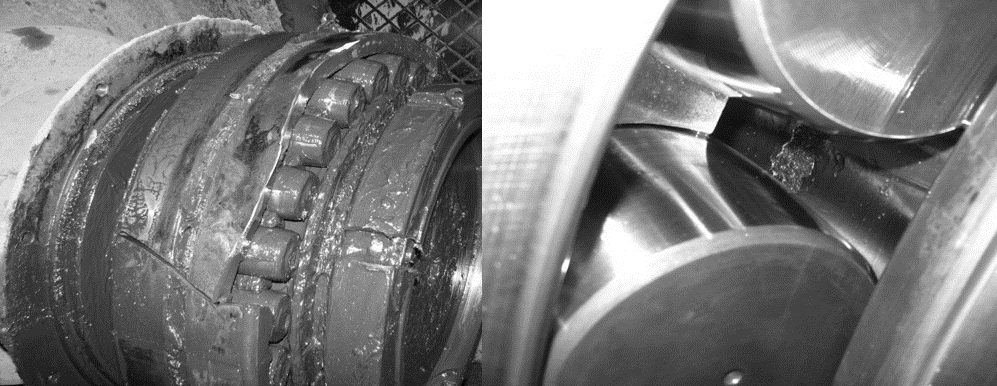
\includegraphics[width = 0.7\textwidth]{wykresy/dmg_race.png}
\caption{Examples of~race damage in~rolling-element bearings, with outer race damage presented on~the~left side, and inner race on~the~right side.}
\label{fig: dmg_race}
\end{figure}

\begin{figure}[ht!]
\centering
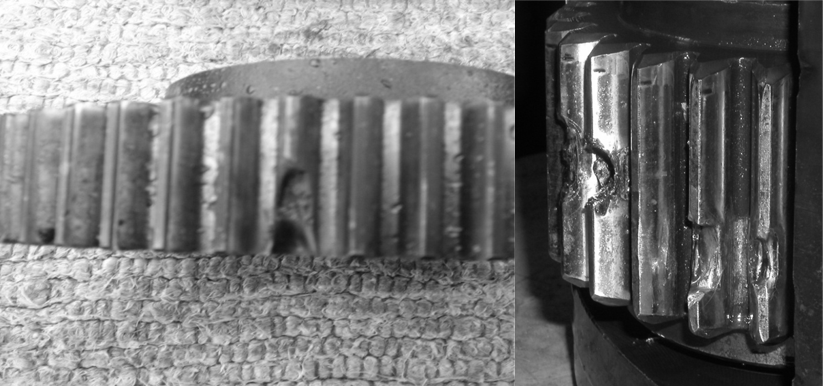
\includegraphics[width = 0.7\textwidth]{wykresy/dmg_tooth.png}
\caption{Examples of~tooth damage in~gearwheels.}
\label{fig: dmg_tooth}
\end{figure}

\begin{figure}[ht!]
\centering
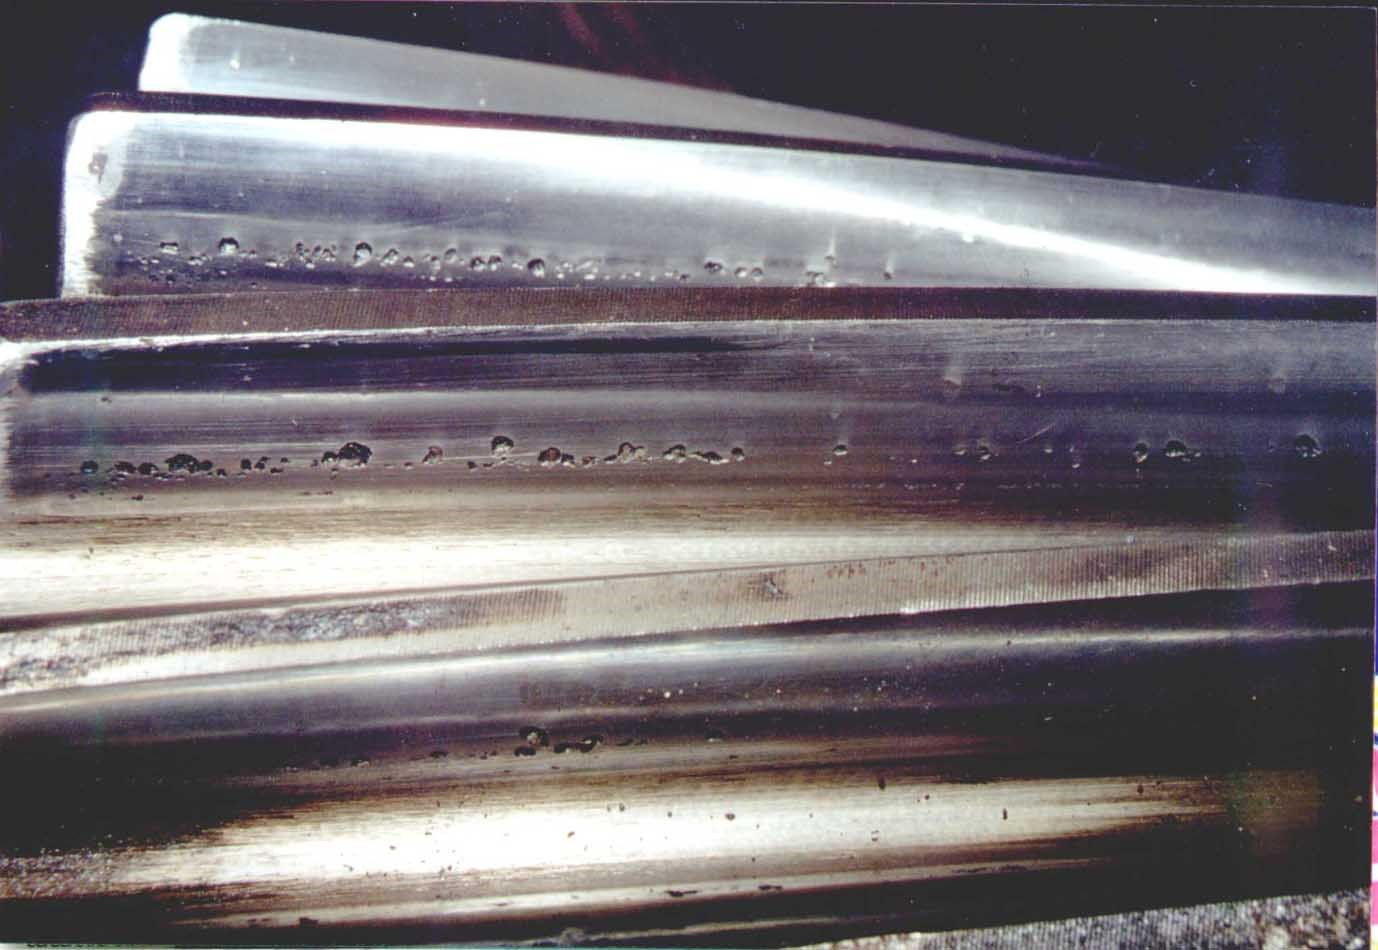
\includegraphics[width = 0.6\textwidth]{wykresy/pitting.jpg}
\caption{Example of~teeth pitting.}
\label{fig: dmg_pit}
\end{figure}

% szumy
Signals generated by~laboratory test rigs will typically include only Gaussian noise. Hence, those signals are expected to~be very easy to~be analyzed, and most of~the~classic techniques are completely enough for conducting investigations in~such conditions. The other type of~signals are the~ones measured in~the~real-life scenarios, and the~feature that distinguishes them from the~laboratory-produced ones is~an~impulsive noise, that can be~expected. It can originate from the~nearby events of~different causes (objects hitting the~machine casing, random disturbances etc.) severely affecting the~overall measurement. 

Vibration signal analysis is~actually one of~the~easiest non-invasive methods of~local damage detection in~machines with rotating elements. Since it~is~sampled relatively frequently in~comparison to~other types of~data measured on~the~industrial machinery, it~can carry a~lot of~important information, especially considering that the~inherent property of~the~operation of~machines with rotating elements is~the~natural occurrence of~cyclic or even periodic behavior. It allows to~use Fourier-based frequency-related analytical mindset as~a~general approach to~processing such type of~data. This feature is~especially convenient due to~the~fact that SOI is~typically connected to~modulations, with special emphasis on~impulsive behavior. 

For the~purpose of~this dissertation an~\emph{impulse} can be~understood as~short-time wideband event in~the~signal, that is~generally caused by~some sort of~impact occurring within a~machine, or being a~result of~an~external event. Such event can be~divided into two general classes: artifacts (i.e. rock or any other arbitrary object hitting a~casing of~the~machine) or impulsive noise (i.e. rock pieces falling into the~crusher).

Impulses as~an~evidence of~a~damage are especially convenient because of~the~idea of~resonant frequency bands (RFB). Resonance is~related to~physical construction and structure of~the~machine, however the~most important fact is~that RFB hardly ever occupies the~entire frequency spectrum of~the~analyzed vibration signal. There are always some bands where signal-to-noise ratio (SNR) is~relatively high, which in~practice means that impulses are possible to~be observed, detected and in~general analyzed in~those bands. Hence, such band (not necessarily continuous) is~called \emph{informative frequency band} (IFB), and its identification is~a~very important approach in~the~field of~machine diagnostics.

\clearpage
\section{Temperature signals from mining machines}

Beside the~main interest in~vibration data, temperature signals have been available for the~author to~be analyzed as~well. During doctoral studies author had an~opportunity to~analyze temperature signals in~two particular cases:

\begin{itemize}
	\item Temperature data from gearboxes in~underground mine belt conveyor driving stations;
	\item Temperature of~engine coolant in~LHD machines operating in~underground mines.
\end{itemize}

On a~large scale of~observation, gearboxes operate in~a~way that it~is~possible to~identify specific patterns within the~measured signal. Since the~machine is~stationary, it~is~easy to~put forth the~interpretation that temperature record of~the~machine can on~some level describe the~character of~its operation. 

Because of~the~fact that on~weekends the~excavation is~stopped, horizontal transportation system is~also shut down, which in~turn allows the~gearboxes to~cool down to~the~level of~ambient temperature. This effect can be~interpreted as~the~first cyclic pattern with a~period of~one week. Another pattern characterized by~the~period of~half a~day is~connected to~the~fact that blasting at~the~mining faces is~performed every 12 hours, which translates into every other work shift. For the~time of~blasting, horizontal transportation system is~also being stopped, which again appears in~the~data as~segments of~clearly decreasing temperature. Third pattern with the~period of~6 hours is~connected to~four work shifts per day. After every shift system is~also stopped, but since this pauses are not as~lengthy as~the~previously mentioned ones, temperature decreases connected to~this process are not manifesting themselves that strongly. One cannot however neglect this effect in~the~assumptions, especially due to~the~fact that it~is~still visible and contributes to~the~overall signal structure.

Considering those three cycles it~is~impossible to~treat this signal as~stationary, especially with respect to~the~mean value. Consequently, methods prepared for the~analysis of~such signal have to~allow nonstationary input, or even assume its cyclostationarity.

Structure of~the~engine coolant temperature measured on~LHD machines is~more complicated and cannot be~analyzed in~terms of~long-term cycles on~the~scale of~days or weeks. In this case shape of~the~signal depends on~many factors, including but not limited to:

\begin{itemize}
	\item Route that the~machine takes at~a~particular shift;
	\item Changes of~the~ambient temperature along the~route when driving from one area to~another;
	\item Operators driving style;
	\item Operation style during a~particular shift (LHD operating with the~support of~hauling truck or not);
	\item Unexpected stoppages during driving;
	\item External human element in~general (presence of~other people or vehicles on~the~route, waiting in~queue for the~dumping screen, other unexpected delays);
	\item Difficulties during loading or unloading;
\end{itemize}

Considering all of~the~uncertainties regarding signal determinism, the~difficulties connected to~the~analysis of~such signal are understandable.

In terms of~temperature data analysis, it~is~easy to~identify overheating as~a~main problem with the~machine. Unfortunately, it~is~defined in~terms of~temperature signal exceeding the~predefined threshold or not. However, such method of~evaluation is~fundamentally incorrect, because temperature data is~fluctuating constantly. Described problem requires methods that do not simply assess the~temperature excess, but take into consideration, e.g. data distributions, signal shapes and structures etc.

\section{The aim of the dissertation}

Based on the analysis of the state of the current knowledge and the personal experience, author presents the following claims:

\begin{itemize}
    \item Utilization of multiple channels of the measurement is a valuable advantage that allows to obtain more complete information than in case of a single-channel measurement. Information in a single channel is very often incomplete or uncertain. Multichannel data enables the information to complement itself between the channels, which improves not only the ease of analysis but also the reliability of the obtained results.
    \item The analysis of multidimensional data representations can provide better insight into the component features or events occurring in the signal. It is especially important considering the fact that very often the sought information is strongly suppressed by high-energy noise present in the real-life measurements. Beside the noise itself, even the components describing the ordinary operation of the machine can make the fault information discovery very difficult.
    \item The most advantageous case happens when a multidimensional diagnostic data is available, and its character allows to utilize multidimensional techniques for detailed investigation of the fault-related signal components.
\end{itemize}

The following work is aimed at addressing the issues imposed by real-life industrial data analysis taking advantage of multiple channels of measurement of diagnostic data, using multidimensional analytical techniques when it is possible, and in the most advantageous cases combine those approaches to maximize the reliability and quality of obtained diagnostic information.